\documentclass[../main.tex]{subfiles}
\begin{document}
\section{Resultados}

Los primeros resultados obtenidos fueron la recreación de los resultados del equipo de Nebraska con el modelo de RFR como lo indicamos en la sección anterior. Los resultados obtuvieron la precisión del trabajo anterior, por lo que se pudo asegurar que los puntos de comienzo fueron exactos para continuar con una búsqueda de alternativas o mejoras. Los siguientes resultados fueron de los modelos de regresión lineal nuevos. En las series de tiempo no se lograron resultados aceptables, pues en cada caso solo se obtiene un promedio de los demás datos para remplazar los datos faltantes (Figure 4).

\begin{figure}[h]
\centering
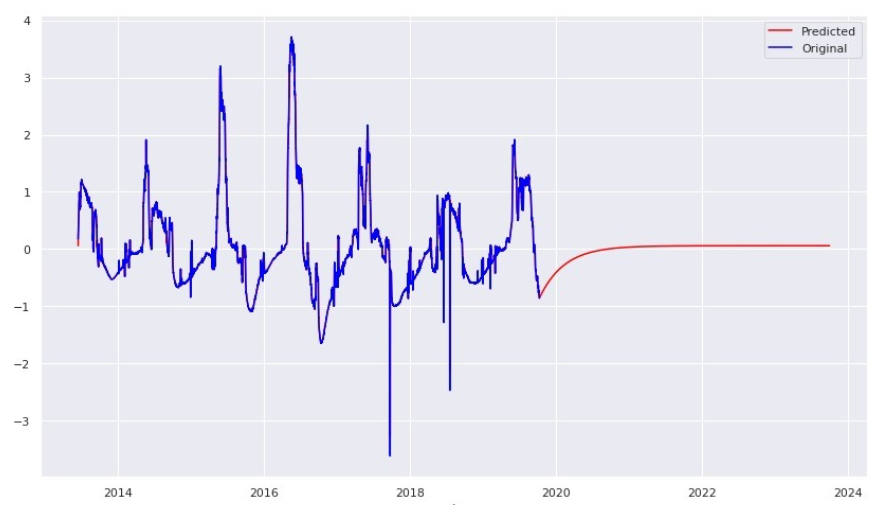
\includegraphics[width=0.8\textwidth]{Fig4}
\caption{Resultados de predicción del nivel del agua con series de tiempo.}
\end{figure}

La variable utilizada para medir su rendimiento fue el MSE (Mean Square Error) y MAE (Mean Absolute Error). Estos representan la distancia del valor verdadero y el promedio del valor obtenido al cuadrado midiendo el error que puede obtener un modelo, mientras que el segundo es el promedio de este valor absoluto. Con esto se observa la precisión del modelo en los resultados tras evaluar sus pérdidas.

Por último se obtuvieron los resultados del modelo convolucional evaluado con las mismas variables, gracias a esto se logró una comparación aceptable (Table 1).

\begin{table}[!h]
\begin{center}
  \begin{tabular}{ | l | l | l | l | l | l | l | l |}
    \hline
      & Lineal & Ridge & Lasso & KNN & Decisión & RFR & CNN\\ \hline
    MSE & 0.784 & 0.245 & 0.443 & 0.195 & 0.398 & 0.398 & 0.143 \\ \hline
    \% MAE & 0.537 & 0.363 & 0.599 & 0.281 & 0.388 & 0.388 & 0.307 \\
    \hline
  \end{tabular}
  \caption{\label cComparación de resultados entre todos los modelos seleccionados.}
\end{center}
\end{table}

Los mejores resultados se obtuvieron en todos los modelos al entrenar los modelos con los datos de una estación específica evaluandolos con esa misma temporada, la única excepción fue el modelo CNN en donde se entrenó con todos los datos y se evaluó por temporada.

Para elegir los mejores resultados se debe tomar en cuenta que aunque KNN muestra mejores resultados de forma general se encontró que estaba sobre entrenado. Esto se observa con que al seleccionar el valor de K el error es muy bajo por lo que no es preciso, mientras que al aumentarlo se dispara el error, dándonos a entender que el error aumentará hasta llegar a un número de K aceptable para el número de datos (Figure 5).

\begin{figure}[h]
\centering
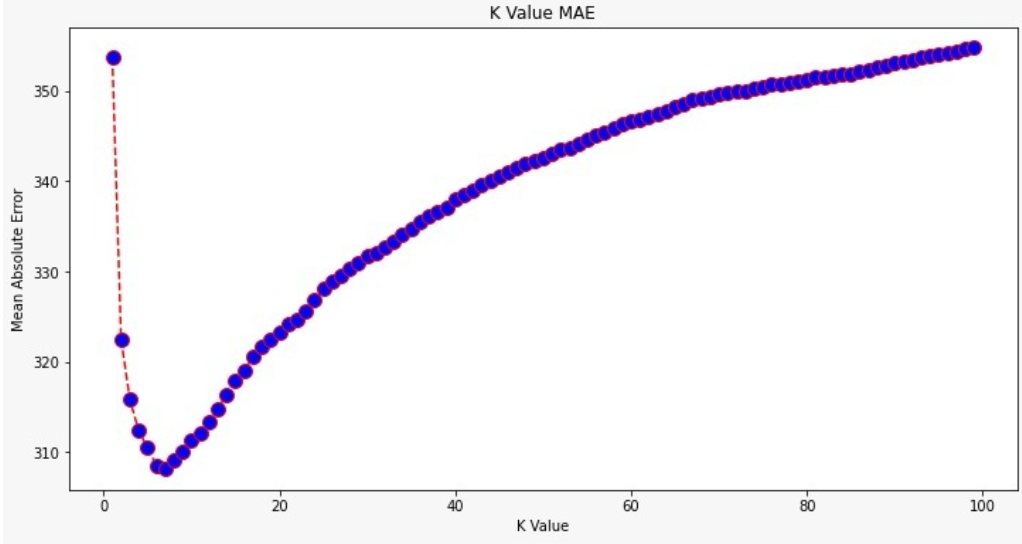
\includegraphics[width=0.8\textwidth]{Fig5}
\caption{Demostración del valor de K a comparación del error.}
\end{figure}

Ya con los resultados obtenidos se logró hacer una comparación en donde se encontró que el modelo de Ridge demostró mejores resultados (Table 2), aunque el modelo de RFR mostró mayor precisión separado por estaciones (Table 3). El modelo CNN no mostraba resultados constantes variando la precisión, aunque en el mejor caso fue el mejor modelo (Table 4), considerando que la fuente de datos fue distinta.

\begin{table}[!h]
\begin{center}
  \begin{tabular}{ | l | l | l | l | l |}
    \hline
     Ridge & Primavera & Verano & Otoño & Invierno \\ \hline
    MSE & 0.423 & 0.332 & 0.475 & 0.797 \\ \hline
    \% MAE & 0.523 & 0.491 & 0.572 & 0.799 \\
    \hline
  \end{tabular}
  \caption{\label cResultados del modelo Ridge separado por temporada.}
\end{center}
\end{table}

\begin{table}[!h]
\begin{center}
  \begin{tabular}{ | l | l | l | l | l |}
    \hline
     RFR & Primavera & Verano & Otoño & Invierno \\ \hline
    MSE & 0.176 & 0.176 & 0.176 & 0.175 \\ \hline
    \% MAE & 0.290 & 0.290 & 0.292 & 0.291 \\
    \hline
  \end{tabular}
  \caption{\label cResultados del modelo RFR separado por temporada.}
\end{center}
\end{table}

\begin{table}[!h]
\begin{center}
  \begin{tabular}{ | l | l | l | l | l |}
    \hline
     CNN & Primavera & Verano & Otoño & Invierno \\ \hline
    MSE & 0.175 & 0.094 & 0.148 & 0.168 \\ \hline
    \% MAE & 0.342 & 0.256 & 0.272 & 0.356 \\
    \hline
  \end{tabular}
  \caption{\label cResultados del modelo CNN separado por temporada.}
\end{center}
\end{table}

\end{document}
\clearpage